\documentclass[oneside, 10pt, notitlepage]{book}
	
	
\usepackage{../_mypackages/monographpreamble}
\usepackage{../_mypackages/commands}

\title{Special Relativity} % \MyTitle
\author{Bruno Murino} % \MyAuthor
\date{\today} % \MyDate

\usepackage{../_mypackages/monographstyle}

\graphicspath{ {figures/} }

%--------------------------------------------------------------------------------------------------

\begin{document}
\frontmatter

\notestp
\dominitoc
% \faketableofcontents
\tableofcontents

\mainmatter

\chapter{The Lorentz Transformation}

Let \(S\) be an inertial frame with coordinates \(x^{\mu}=(ct=x^0,x_1,x^2,x^3)\) and let \(S{\prime}\) be an inertial frame be moving with speed \(v\) along the \(x^1\) axis of \(S\), with coordinates \(x{\prime}^{\mu} = (ct{\prime}=x{\prime}^0, x{\prime}^1,x{\prime}^2,x{\prime}^3)\). Let event A happen, with respect to \(S\) at \((ct_A = x_A^0,x_A^1,x_A^2,x_A^3)\). Let the frames coincide at \(t=t{\prime}=0\) Then this same event happened, with respect to \(S{\prime}\), at
\begin{subequations}
    \begin{align}[left = \empheqlbrace\,]
    & x_A{\prime}^0 = \gamma(v)\lr{x_A^0 - \beta x_A^1} \\
	& x_A{\prime}^1 = \gamma(v)\lr{x_A^1 - \beta x_A^0} \\
	& x_A{\prime}^2 = x_A^2 \\
	& x_A{\prime}^3 = x_A^3
    \end{align}
\end{subequations}
where \(\beta = v/c\) and \(\gamma(v) = (1-\beta^2)^{-1/2} \geq 1\) is the so called \emph{Lorentz factor}.  

There is a quantity that is preserved upon Lorentz transformations, the so called \emph{invariant interval}
\begin{equation}
    \Delta s^2 = (c\Delta t)^2 - (\Delta x^1)^2 - (\Delta x^2)^2 - (\Delta x^3)^2 = (c\Delta t)^2 - (\Delta \vb{x})^2
\end{equation}
which means that if \(t{\prime}\), \(x{\prime}^1\), \(x{\prime}^2\), \(x{\prime}^3\) are Lorentz transformed coordinates, the invariant interval is written as
\begin{equation}
    \Delta s{\prime}^2 = (c\Delta t{\prime})^2 - (\Delta x{\prime}^1)^2 - (\Delta x{\prime}^2)^2 - (\Delta x{\prime}^3)^2
\end{equation}
and satisfies
\begin{equation}
    \Delta s^2 = \Delta s{\prime}^2
\end{equation}
  

\section{Properties of \texorpdfstring{$\gamma(v)$}{gamma of v}}

The \(\gamma(v)\) is defined as 
\begin{equation}
    \gamma(v) = \frac{1}{\sqrt{1-\beta^2}} \qq{with} \beta = v/c
\end{equation}
  

We have the identity
\begin{equation}\gamma v = c \sqrt{\gamma^2 - 1}\end{equation}
\begin{proof}
	\begin{equation}\gamma v = c \sqrt{\gamma^2 - 1}\end{equation}
	\begin{equation}\gamma^2 v^2 = c^2 \lr{\gamma^2 - 1}\end{equation}
	\begin{equation}\gamma^2 \beta^2 = \gamma^2 - 1\end{equation}
	\begin{equation}\gamma^2 -\gamma^2 \beta^2 = 1\end{equation}
	\begin{equation}\gamma^2 \lr{1 - \beta^2} = 1\end{equation}
	\begin{equation}\gamma^2 = \frac{1}{1-\beta^2}\end{equation}
	Which is immediate from the definition.
\end{proof}

We also have the identity 
\begin{equation}\dv{\gamma}{v} = \frac{\gamma^3 v}{c^2}\end{equation}
\begin{proof}
	First lets write \(\gamma\) as 
	\begin{equation}\gamma(v) = \lr{1-v^2/c^2}^{-1/2}\end{equation}
	From the chain rule: 
	\begin{equation}\dv{\gamma}{v} = \lr{-\frac{1}{2}}\lr{1-v^2/c^2}^{-3/2}\lr{-\frac{1}{c^2}}\lr{2v}\end{equation}
	\begin{equation}\dv{\gamma}{v} = \lr{\lr{1-v^2/c^2}^{-1/2}}^3 \frac{v}{c^2} = \frac{\gamma^3 v}{c^2}\end{equation}
\end{proof}

Finally, we have the identity 
\begin{equation}\dv{(\gamma v)}{v} = \gamma^3\end{equation}
\begin{proof}
	First, from the product rule 
	\begin{equation}\dv{(\gamma v)}{v} = \dv{\gamma}{v} v + \gamma \dv{v}{v} = \dv{\gamma}{v} v + \gamma \end{equation}
	so we need to find \(\dv*{\gamma}{v}\). But we already know that
	\begin{equation}\dv{\gamma}{v} = \frac{\gamma^3 v}{c^2}\end{equation}
	so we have 
	\begin{equation}\dv{(\gamma v)}{v} = \dv{\gamma}{v} v + \gamma = \frac{\gamma^3 v}{c^2} v + \gamma\end{equation}
	\begin{equation}\dv{(\gamma v)}{v} = \gamma^3 \beta^2 + \gamma = \gamma \lr{\gamma^2 \beta^2 + 1}\end{equation}
	But since we know that, from the definition,
	\begin{equation}\gamma^2 \lr{1-\beta^2} = 1\end{equation}
	we find that
	\begin{equation}\gamma^2 \beta^2 + 1 = \gamma^2\end{equation}
	which finally leads us to 
	\begin{equation}\dv{(\gamma v)}{v} = \gamma \lr{\gamma^2 \beta^2 + 1} = \gamma (\gamma^2)\end{equation}
	Thus
	\begin{equation}\dv{(\gamma v)}{v} = \gamma^3\end{equation}

\end{proof}

\section{Rapidity}

The \emph{rapidity} \(\phi\) is defined by
\begin{equation}\tanh \phi = \beta \end{equation}
thus it has the following property
\begin{equation}\cosh \phi \pm \sinh \phi = \exp{\pm \phi}\end{equation}
besides the usual hyperbolic functions properties
\begin{equation}\tanh \phi = \frac{\sinh \phi}{\cosh \phi}\end{equation}
\begin{equation}\cosh^2 \phi - \sinh^2 \phi = 1\end{equation}
\begin{equation}\cosh \phi = \cos (i\phi)\end{equation}
\begin{equation}\sinh \phi = -i \sin (i \phi)\end{equation}
  

Lets demonstrate some further properties.

\begin{enumerate}
    \item \begin{equation}\cosh \phi = \gamma\end{equation}
        \begin{proof}
        	\begin{equation}\tanh \phi = \beta\end{equation}
            \begin{equation}\frac{\sinh \phi}{\cosh \phi} = \beta\end{equation}
            \begin{equation}\cosh^2 \phi = \frac{\sinh^2 \phi}{\beta^2}\end{equation}
            but
            \begin{equation}\sinh^2 \phi = \cosh^2 \phi -1\end{equation}
            then
            \begin{equation}\cosh^2 \phi = \frac{\cosh^2 \phi -1}{\beta^2} = \frac{\cosh^2 \phi}{\beta^2} - \frac{1}{\beta^2}\end{equation}
        	\begin{equation} \cosh^2 \phi \lr{1 - \frac{1}{\beta^2}} = - \frac{1}{\beta^2} \end{equation}
        	\begin{equation}\cosh^2 \phi \lr{\frac{1}{\beta^2} - 1} = \frac{1}{\beta^2}\end{equation}
        	\begin{equation}\cosh^2 \phi  = \frac{1}{\lr{\frac{1}{\beta^2} - 1}\beta^2} = \frac{1}{1-\beta^2} = \gamma^2\end{equation}
        	thus
        	\begin{equation}\cosh \phi = \gamma\end{equation}
        \end{proof}
        
    \item \begin{equation}\sinh \phi = \beta \gamma\end{equation}
        \begin{proof}
        	\begin{equation}\tanh \phi = \beta\end{equation}
            \begin{equation}\frac{\sinh \phi}{\cosh \phi} = \beta\end{equation}
            \begin{equation}\sinh \phi = \beta \cosh \phi = \beta \gamma\end{equation}
        \end{proof}
 
    \item \begin{equation}\exp{\phi} = \lr{\frac{c+v}{c-v}}^{1/2} = \lr{\frac{1+\beta}{1-\beta}}^{1/2}\end{equation}
        \begin{proof}
        	\begin{equation}\exp{\phi} = \cosh \phi + \sinh \phi \end{equation}
        	\begin{equation}\exp{\phi} = \gamma + \gamma \beta \end{equation}
        	\begin{equation}\exp{\phi} = \gamma(1+\beta) = \frac{1+\beta}{\sqrt{1-\beta^2}}\end{equation}
        	\begin{equation}\exp{\phi} = \sqrt{ \frac{(1+\beta)^2}{1-\beta^2} }\end{equation}
        	\begin{equation}\exp{\phi} = \sqrt{ \frac{(1+\beta)(1+\beta)}{(1+\beta)(1-\beta)}  }\end{equation}
        	thus
        	\begin{equation}\exp{\phi} = \lr{\frac{1+\beta}{1-\beta}}^{1/2}\end{equation}
        \end{proof}
        
        
        
    \item We can write
        \begin{equation}x{\prime}= \gamma (x - \beta ct) \qq{and} ct{\prime} = \gamma (ct - \beta x)\end{equation}
        as
        \begin{equation}x{\prime}= x \cosh \phi - ct \sinh \phi \qq{and} ct{\prime} = ct \cosh \phi - x \sinh \phi\end{equation}
        \begin{proof}
        	\begin{equation}x{\prime}= \gamma (x - \beta ct) = \gamma x - \gamma \beta ct\end{equation}
            \begin{equation}x{\prime}= \cosh \phi x - \sinh \phi ct\end{equation}
            thus
            \begin{equation}x{\prime}= x \cosh \phi - ct \sinh \phi\end{equation}
            Also
            \begin{equation}ct{\prime} = \gamma (ct - \beta x) = \gamma ct - \gamma \beta x\end{equation}
            \begin{equation}ct{\prime} = \cosh ct - \sinh x\end{equation}
            thus
            \begin{equation}ct{\prime} = ct \cosh \phi - x \sinh \phi\end{equation}
        \end{proof}
        
        
        
    \item We can write 
        \begin{equation}ct{\prime}+ x{\prime}= \exp{-\phi} (ct + x) \qq{and} ct{\prime} - x{\prime} = \exp{\phi} (ct - x) \end{equation}
        \begin{proof}
        	\begin{equation}ct{\prime}+ x{\prime} = (ct \cosh \phi - x \sinh \phi) + (x \cosh \phi - ct \sinh \phi)\end{equation}
        	\begin{equation}ct{\prime}+ x{\prime} = \cosh \phi (ct + x) - \sinh \phi (ct + x)\end{equation}
        	\begin{equation}ct{\prime} + x{\prime}= (\cosh \phi - \sinh \phi)(ct+x)\end{equation}
        	\begin{equation}ct{\prime}+ x{\prime}= \exp{-\phi}(ct+x)\end{equation}
        	Also
        	\begin{equation}ct{\prime}- x{\prime} = (ct \cosh \phi - x \sinh \phi) - (x \cosh \phi - ct \sinh \phi)\end{equation}
        	\begin{equation}ct{\prime}+ x{\prime} = \cosh \phi (ct - x) + \sinh \phi (ct - x)\end{equation}
        	\begin{equation}ct{\prime} + x{\prime}= (\cosh \phi + \sinh \phi)(ct-x)\end{equation}
        	\begin{equation}ct{\prime}+ x{\prime}= \exp{\phi}(ct-x)\end{equation}
        \end{proof}

    \item If our coordinates are
        \begin{equation}\xi = ct+x \qq{and} \zeta = ct-x\end{equation}
        then
        \begin{equation}\xi{\prime} = \exp{-\phi}\xi\end{equation}
        \begin{equation}\zeta{\prime} = \exp{\phi}\zeta\end{equation}
        And since \(\exp{\phi}\geq1\) while \(\exp{-\phi}\leq1\), the axis don't rotate (as the \(x\) and \(ct\) would), but the \(\xi\) axis shrinks while the \(\zeta\) axis expands.  
        
        The invariant interval on \(x\) and \(t\) coordinates is
        \begin{equation}\lr{\Delta s}^2 = \lr{c\Delta t}^2 - \lr{\Delta x}^2\end{equation}
        but how it is on \(\xi\) and \(\zeta\) coordinates? Let A and B be two events, then
        \begin{equation}\xi{\prime}_A = ct{\prime}_A + x{\prime}_A = \exp{-\phi}\xi_A\end{equation}
        \begin{equation}\zeta{\prime}_A = ct{\prime}_A - x{\prime}_A = \exp{\phi}\zeta_A\end{equation}
        and
        \begin{equation}\xi{\prime}_B = ct{\prime}_B + x{\prime}_B = \exp{-\phi}\xi_B\end{equation}
        \begin{equation}\zeta{\prime}_B = ct{\prime}_B - x{\prime}_B = \exp{\phi}\zeta_B\end{equation}
        Making \(\xi{\prime}_B - \xi{\prime}_A\) and the same for \(\zeta{\prime}\) we find
        \begin{equation}\xi{\prime}_B - \xi{\prime}_A = \Delta \xi{\prime} = c \Delta t{\prime} + \Delta x{\prime} = \exp{-\phi}\Delta \xi\end{equation}
        \begin{equation}\zeta{\prime}_B - \zeta{\prime}_A = \Delta \zeta{\prime} = c \Delta t{\prime} - \Delta x{\prime}= \exp{\phi}\Delta \zeta\end{equation}
        and multiplying one by the other we find
        \begin{equation}\Delta \xi{\prime} \Delta \zeta{\prime} = \Delta \xi \Delta \zeta\end{equation}
        which is exactly the same as
        \begin{equation}\lr{c\Delta t{\prime}}^2 - \lr{\Delta x{\prime}}^2 = \lr{c\Delta t}^2 - \lr{\Delta x}^2 \end{equation}
        which is just
        \begin{equation}\lr{\Delta s}^2=\lr{\Delta s{\prime}}^2\end{equation}
        thus
        \begin{equation}\lr{\Delta s}^2 = \Delta \xi \Delta \zeta\end{equation}
        
        
    \item Rapidity is aditive under colinear speeds.










\end{enumerate}







\section{Order of events}

Let A and B be two events. With respect to \(S\), they happened at \((x_A^0,x_A^1,x_A^2,x_A^3)\) and \((x_B^0,x_B^1,x_B^2,x_B^3)\), respectively. Assume that \(x_A^0 - x_B^0 \leq 0\), meaning that, with respect to \(S\), A happened before B in time, or at the same time, and that \(x_A^1 - x_B^1 \leq 0\), meaning that B happened further from the origin than A. Then, with respect to \(S{\prime}\), their position in time is
\begin{equation}x_A{\prime}^0 = \gamma(v)\lr{x_A^0 - \beta x_A^1}\end{equation}
\begin{equation}x_B{\prime}^0 = \gamma(v)\lr{x_B^0 - \beta x_B^1}\end{equation}
which implies that 
\begin{equation}x_A{\prime}^0-x_B{\prime}^0 = \gamma(v)\lr{(x_A^0-x_B^0) - \beta (x_A^1-x_B^1)}\end{equation}
If we want the order of events to be kept, we need that 
\begin{equation}x_A{\prime}^0-x_B{\prime}^0 = \gamma(v)\lr{(x_A^0-x_B^0) - \beta (x_A^1-x_B^1)}\leq0\end{equation}
since \(\gamma \geq 1\), we only need 
\begin{equation}(x_A^0-x_B^0) - \beta (x_A^1-x_B^1)\leq0\end{equation}
thus
\begin{equation}(x_A^0-x_B^0) \leq \beta (x_A^1-x_B^1)\end{equation}
Lets orient the frames in a way that the position of the events differ only with respect to the \(x^0\) and \(x^1\) coordinate (we can do that since we are considering only two events), that \(x_A^0=0\) (\(t_A=0\)) and that \(x_A^1 = 0\) (event A at the origin of \(S\)). Notice that the \(S{\prime}\) still moves along the \(x^1\) axis with speed \(v\). We want this frame, with respect to \(S\), to depart from A at \(x^0 = x_A^0\) and reach \(x_B^1\) when \(x^0 = x_B^0\), thus we want the frame to move with speed \(v = (x_B^1 - x_A^1)/(t_B - t_A)\), or \(\beta = (x_B^1 - x_A^1)/(x_B^0 - x_A^0)\). Now, our condition that maintains the order of events is 
\begin{equation}1 \geq \beta \frac{(x_B^1-x_A^1)}{(x_B^0-x_A^0)} = \beta^2\end{equation}
thus
\begin{equation}\beta^2 \leq 1 \qq{implying} \beta \leq 1 \qq{then} v \leq c\end{equation}
meaning that the required speed of the signal must not surpass the speed of light \(c\). So if the signal that connects the events has speed less than or equal \(c\), the order of the events is always the same for every inertial frame.  


\subsection{Same place events}

If, with respect to an inertial frame \(S\), two events happen on the same place, the connecting signal must have speed \(0\) (zero), which is less than \(c\), allowing us to conclude that the order of events will always be kept, so 
\begin{equation}\sgn(\Delta t{\prime}) = \sgn(\Delta t)\end{equation}
  

Let \(S{\prime}\) be a moving inertial frame with respect to \(S\). Then the invariance of the invariant interval is stated as 
\begin{equation}(c\Delta t)^2 - (\Delta \vb{x})^2 = (c\Delta t{\prime})^2 - (\Delta \vb{x}{\prime})^2\end{equation}
but if the events happen on the same place with respect to \(S\), it follows that \(\Delta \vb{x} = 0\), thus 
\begin{equation}(\Delta t)^2 = (\Delta t{\prime})^2 - \lr{\frac{\Delta \vb{x}{\prime}}{c}}^2\end{equation}
which implies that
\begin{equation}(\Delta t{\prime})^2 \geq (\Delta t)^2\end{equation}
and since we don't need to worry about the sings changing, we can take the square root of both sides to obtain
\begin{equation}\Delta t{\prime} \geq \Delta t\end{equation}
which means that the temporal distance between two events that happened on the same place with respect to \(S\), is always greater than or equal when measured with respect to a moving frame \(S{\prime}\).  


\subsection{Same time events}

Let two events A and B happen at the same time with respect to a frame \(S\), and let \(S{\prime}\) be a moving inertial frame with respect to \(S\). Then the invariance of the invariant interval can be stated as 
\begin{equation}(\Delta \vb{x})^2 = (\Delta \vb{x}{\prime})^2 -(c\Delta t{\prime})^2\end{equation}
implying that
\begin{equation} (\Delta \vb{x}{\prime})^2 \geq (\Delta \vb{x})^2\end{equation}
thus 
\begin{equation}\abs{\Delta \vb{x}{\prime}} \geq \abs{\Delta \vb{x}}\end{equation}
which means that the spatial distance with respect to \(S\) between two events that happened at the same time with respect to \(S\) is smaller than or equal the spatial distance with respect to a moving frame \(S{\prime}\).  


\section{Length contraction}

The length of an object is determined by the distance between its endpoints at the same time. Therefore, to measure how length is affected by relativity, we must measure, at the same time, the distance between the object's endpoints with respect to a moving frame.  

Let \(S\) an inertial frame and let \(S{\prime}\) be an inertial frame moving with respect to \(S\) along the \(x^1\) axis of \(S\) with speed \(v\). Let a rod be placed at rest with one endpoint A at \(x_A\) of \(S\) and the other endpoint B at \(x_B\), meaning that, with respect to \(S\), the length of the rod is \(x_B - x_A \equiv L_0\). In this case, the \(y\) and \(z\) coordinates on both frames are irrelevant. Let the measurement of the position of the endpoint A be the A event and the measurement of the position of the endpoint B be the B event. Both events must occur at the same time, so \(t_A = t_B = t\).

To find the length of the rod with respect to \(S{\prime}\), we must measure the position of both its endpoints at the same time, thus \(x_A{\prime}\) and \(x_B{\prime}\) must be measured at \(t{\prime}\). But these points, whatever they are, must match \(x_A\) and \(x_B\) at \(t\) with respect to \(S\). This points \(x_A{\prime}\) and \(x_B{\prime}\) can be calculated by computing the inverse Lorentz transformation:
\begin{equation}x_A = \gamma(x_A{\prime} + v t{\prime})\end{equation}
\begin{equation}x_B = \gamma(x_B{\prime} + v t{\prime})\end{equation}
When we make \(\gamma(x_A{\prime} + v t{\prime})\) be \(x_A\) and \(\gamma(x_B{\prime} + v t{\prime})\) be \(x_B\), we ensure that \(x_A\) and \(x_B\) are simultaneous. Since \(L_0 = x_B - x_A\), we find that
\begin{equation}L_0 = \gamma(x_B{\prime} + v t{\prime}) - \gamma(x_A{\prime} + v t{\prime}) = \gamma(x_B{\prime} - x_A{\prime}) = \gamma L{\prime}\end{equation}
thus
\begin{equation}L{\prime} = \frac{L_0}{\gamma}\end{equation}
Since \(\gamma \geq 1\), it follows \(L{\prime}\leq L_0\), thus the name Lorentz contraction.  

\subsection{Change of angle}

Let a rod be inclined \(\alpha\) degrees with respect to the \(x\) axis of an inertial frame \(S\). Let \(L_x\) be the projection of the rod along the \(x\) axis and analogous for \(L_y\). Then
\begin{equation}\frac{L_y}{L_x} = \tan(\alpha)\equiv m\end{equation}
If \(S{\prime}\) is an inertial frame moving along the \(x\) axis with speed v, the lengths along \(x\) will suffer Lorentz contraction, meaning that the length of \(L_x\) with respect to \(S{\prime}\) will be
\begin{equation}L_x{\prime} = \frac{L_x}{\gamma}\end{equation}
Since nothing happens with the \(y\) axis, \(L_y\) remains the same for both \(S\) and \(S{\prime}\), meaning that \(L_y{\prime} = L_y\). Thus the new inclination \(\alpha{\prime}\) is given by
\begin{equation}
m{\prime}= \tan(\alpha{\prime}) = \frac{L_y{\prime}}{L_x{\prime}} = \frac{L_y}{L_x/\gamma} = \gamma \frac{L_y}{L_x} = \gamma m\end{equation}


\section{Time dilation}

One way to deduce time dilation is the following.  

Consider a pair of mirrors spaced \(d\) and a light signal going from one to the other. How long it takes for a signal to leave a mirror and get back to it? The signal have speed \(c\), of course, and the distance it travels is \(2d\), so
\begin{equation}\label{eq:timedilationDt}
\Delta t = \frac{2d}{c}
\end{equation}
This is frame \(S\).  

Let \(S{\prime}\) be a frame moving parallel to the mirrors with speed \(v\), moving away from the signal. Let the frames coincide at \(t=t{\prime}=0 \). From \(S{\prime}\) perspective, the signal is moving away with horizontal speed \(v\), so when a signal takes \(\Delta t{\prime}\) to reach a mirror again, it travels \(v \Delta t{\prime}\) horizontally from the origin. Figure \ref{fig:timedilation} should make the situation a bit more clear.  

\begin{figure}[t]
\caption{Time dilation situation.}
\centering
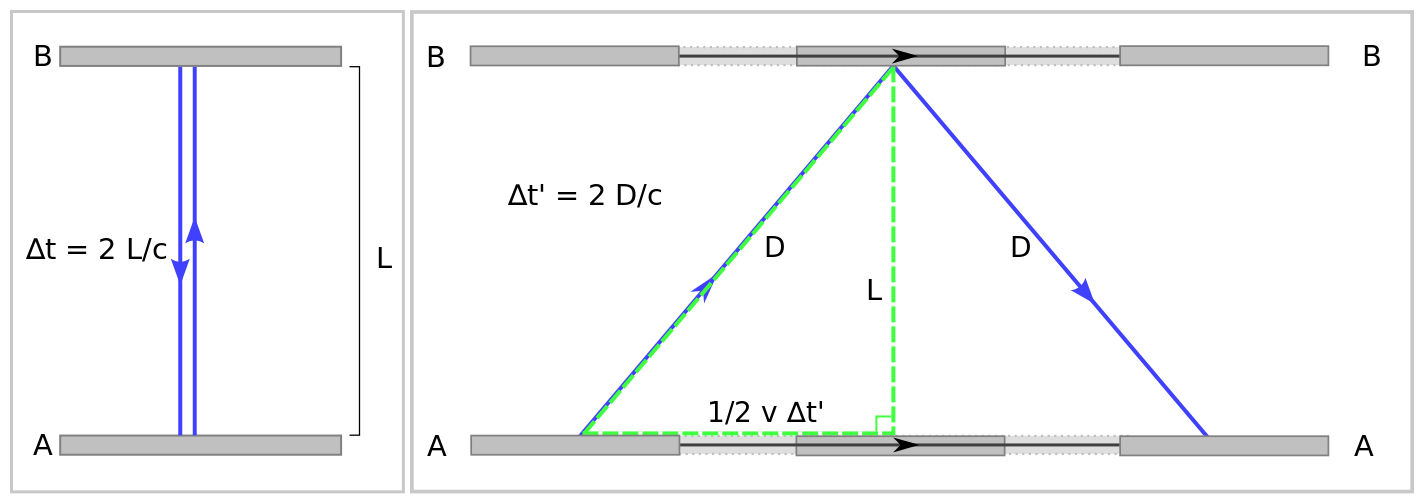
\includegraphics[width=\textwidth]{timedilation}
\label{fig:timedilation}
\end{figure}

From the perspective of the moving frame, the total length travelled by the light signal is \(2D\), with speed \(c\), implying that it took
\begin{equation}\label{eq:timedilationDtprime}
\Delta t{\prime}= \frac{2D}{c}
\end{equation}
to happen. From figure \ref{fig:timedilation} we can see a triangle for which we can apply the Pythagorean theorem to find \(D\)
\begin{equation}\label{eq:timedilationPythag}
\lr{D}^2 = d^2 + \lr{\frac{v \Delta t{\prime}}{2}}^2 \qq{thus} \lr{2D}^2 = \lr{2d}^2 + \lr{v \Delta t{\prime}}^2
\end{equation}
Plugging \(2D\) from \eqref{eq:timedilationDtprime} and \(2d\) from \eqref{eq:timedilationDt} on \eqref{eq:timedilationPythag} we find that
\begin{equation}(c\Delta t{\prime})^2 = (c \Delta t)^2 + v^2 (\Delta t{\prime})^2\end{equation}
which we can manipulate to find
\begin{equation}\lr{\frac{\Delta t}{\Delta t{\prime}}}^2 = \frac{c^2 - v^2}{c^2} = \frac{1}{\gamma^2}\end{equation}
meaning that
\begin{equation}\Delta t{\prime} = \gamma \Delta t\end{equation}
and since \(\gamma \geq 1\), \(\Delta t{\prime} \geq \Delta t \), hence time dilation.  


\section{Wave equation}

Lets demonstrate that the wave equation is invariant under Lorentz transformations.  
Let \(S\) be a frame at rest whose coordinates are \((ct,x,y,z)\) and let \(S{\prime}\) be a frame moving along the \(x\)-axis of \(S\), with speed \(v\) (away from \(S\)), with coordinates \((ct{\prime},x{\prime},y{\prime},z{\prime})\) such that
\begin{subequations}
    \begin{align}[left = \empheqlbrace\,]
    & t{\prime} = \gamma\lr{t - \frac{v}{c^2} x} \\
	& x{\prime} = \gamma\lr{x - v t} \\
	& y{\prime} = y \\
	& z{\prime} = z
    \end{align}
\end{subequations}

The wave equation is
\begin{equation}
\lr{\pdv[2]{x} + \pdv[2]{y} + \pdv[2]{z} - \frac{1}{c^2}\pdv[2]{t}}\Psi = 0
\end{equation}
so we need first find the corresponding derivatives on \(S{\prime}\). Since \(y=y{\prime}\) and \(z=z{\prime}\), we don't need to worry about this coordinates. Lets start
\begin{equation}\pdv{x} = \pdv{x{\prime}}{x}\pdv{x{\prime}} + \pdv{t{\prime}}{x}\pdv{t{\prime}}  \end{equation}
since \(\pdv*{x{\prime}}{x} = \gamma \) and \(\pdv*{t{\prime}}{x} = -\gamma v/c^2\)
we have
\begin{equation}\pdv{x} = \gamma \pdv{x{\prime}} - \frac{\gamma v}{c^2}\pdv{t{\prime}}\end{equation}
Thus if
\begin{equation}\pdv[2]{x} = \pdv{x} \lr{\pdv{x}}\end{equation}
it also follows that
\begin{equation}\pdv[2]{x} = \lr{\gamma \pdv{x{\prime}} - \frac{\gamma v}{c^2}\pdv{t{\prime}}}\lr{\gamma \pdv{x{\prime}} - \frac{\gamma v}{c^2}\pdv{t{\prime}}}\end{equation}
which gives us
\begin{equation}\pdv[2]{x} = \gamma^2 \pdv[2]{x{\prime}} -2 \frac{\gamma^2 v}{c^2}\pdv{}{x{\prime}}{t{\prime}} +\frac{{\gamma^2} {v^2}}{c^4} \pdv[2]{t{\prime}}\end{equation}
On the other hand, for the time derivative we find
\begin{equation}\pdv{t} = \pdv{t{\prime}}{t}\pdv{t{\prime}} + \pdv{x{\prime}}{t}\pdv{x{\prime}} = \gamma \pdv{t{\prime}} - \gamma v \pdv{x{\prime}}\end{equation}
thus
\begin{equation}\pdv[2]{t} = \gamma^2 \pdv{t{\prime}} - 2 \gamma^2 v \pdv{}{x{\prime}}{t{\prime}} + \gamma^2 v^2 \pdv[2]{x{\prime}}\end{equation}
Plugging this equalities on the wave equation we find that
\begin{equation}
\begin{split}
\pdv[2]{x} - \frac{1}{c^2}\pdv[2]{t}=\gamma^2 \pdv[2]{x{\prime}} -2 \frac{\gamma^2 v}{c^2}\pdv{}{x{\prime}}{t{\prime}} &+\frac{{\gamma^2} {v^2}}{c^4} \pdv[2]{t{\prime}} -\\
& \frac{1}{c^2}\lr{\gamma^2 \pdv{t{\prime}} - 2 \gamma^2 v \pdv{}{x{\prime}}{t{\prime}} + \gamma^2 v^2 \pdv[2]{x{\prime}}} \\
&= \lr{\gamma^2 - \frac{\gamma^2 v^2}{c^2}}\pdv[2]{x{\prime}} - \lr{\gamma^2 - \frac{\gamma^2 v^2}{c^2}}\frac{1}{c^2}\pdv[2]{t{\prime}}
\end{split}
\end{equation}
and since
\begin{equation}\gamma^2 = \frac{1}{1-\frac{v^2}{c^2}} \qq{implying} \gamma^2 - \frac{\gamma^2 v^2}{c^2}=1\end{equation}
it follows that
\begin{equation}\pdv[2]{x} - \frac{1}{c^2}\pdv[2]{t} = \pdv[2]{x{\prime}} - \frac{1}{c^2}\pdv[2]{t{\prime}}\end{equation}
which means that the wave equation on the \(S\) frame and on the \(S{\prime}\) frame is the same, thus, it is invariant under Lorentz transformations. 

\section{Ladder Paradox or Pole in Barn Paradox}

Consider a ladder with proper length 10 meters and a barn with proper depth 5 meters. We'll try to fit the ladder (horizontally) in the barn (we want 10 meters to fit in 5 meters).

Let \(S\) be the frame of the ladder and \(S{\prime}\) be the frame of the barn. The ladder approaches the barn with speed \(v\). 

From the perspective of the barn (\(S{\prime}\)), the ladder is moving with speed \(v\), therefore it suffer Lorentz contraction. How much should the speed \(v\) be, so that the barn perceives the length of the ladder as 5 meters?  
Well, Lorentz contraction says that the length perceived is equal to the proper length divided by the Lorentz factor (\(\gamma\)), so
\begin{equation}L_{\text{ladder perceived}} = \frac{L_{\text{ladder proper}}}{\gamma}\end{equation}
The proper length of the ladder is 10 meters, and the barn wants to perceive it as 5 meters, so \(\gamma\) should be
\begin{equation}\gamma = \frac{L_{\text{ladder proper}}}{L_{\text{ladder perceived}}} = \frac{10}{5} = 2\end{equation}
If \(\gamma = 2\)
\begin{equation}\gamma^2 = 4 = \frac{1}{1-\beta^2} \qq{thus} \beta = \frac{\sqrt{3}}{2}\end{equation}
So the ladder must be approaching the barn with \(\beta = \sqrt{3}/2\). On this case, since both the ladder and the barn have the same size (5 meters), from the barn perspective the ladder will fit!  

On the other hand, with respect to the ladder frame, the \emph{barn} is approaching with \(\beta = \sqrt{3}/2\), thus the \emph{barn} suffers Lorentz contraction! For the ladder, the barn has length
\begin{equation}L_{\text{barn perceived}} = \frac{L_{\text{barn proper}}}{\gamma=2} = \frac{5}{2} = 2.5 \qq{meters}\end{equation}
Which means that, from the ladder perspective, the ladder won't ever fit in the barn, since the ladder is 10 meters long while the barn is 2.5 meters deep, hence the paradox!  

To solve this apparent paradox, we can consider three events:
\begin{enumerate}
    \item The front of the ladder enters the barn.
    \item The back of the ladder enters the barn.
    \item The front of the ladder reached the end of the barn.
\end{enumerate}
Let the frame \(S\) (ladder) be centred at the front of the ladder and the frame \(S{\prime}\) be centred and the entrance of the barn. Let the events (1), (2) and (3) happen respectively at \(t_1\),\(t_2\) and \(t_3\) with respect to the ladder and similar with respect to the barn. Let \(t_1=t{\prime}_1=0\) so the frames coincide when event (1) takes place.  

\subsection{The barn perspective}

From the barn perspective recall that both the ladder and the barn have 5 meters.  

At instant \(t{\prime}_1\) the back of the ladder is 5 meters away from the entrance of the barn, so at \(t{\prime}_2\) the back of the ladder moved 5 meters with speed \(\beta = \sqrt{3}/2\). Since
\begin{equation}t{\prime}_2 - t{\prime}_1 = \frac{L_{\text{ladder perceived}}}{v}\end{equation}
we find that
\begin{equation}t{\prime}_2 = \frac{10 \sqrt{3}}{3c} \text{seconds}\end{equation}


At instant \(t{\prime}_1\) the front of the ladder is at the origin, at the entrance of the barn. At instant \(t{\prime}_3\) the front of the ladder moved all the way to the end of the barn, that is 5 meters deep, with speed \(\beta = \sqrt{3}/2\). So the front of the ladder moved 5 meters on the interval \(t{\prime}_3 - t{\prime}_1\). Since
\begin{equation}t{\prime}_3 -t{\prime}_1 = \frac{L_{\text{barn proper}}}{v} \end{equation}
we find that
\begin{equation}t{\prime}_3 = \frac{10 \sqrt{3}}{3c} \text{seconds}\end{equation}


Since \(t{\prime}_2 = t{\prime}_3\), events (2) and (3) happen simultaneously with respect to the barn.

\subsection{The ladder perspective}

From the ladder perspective recall that the ladder is 10 meters long and the barn is 2.5 meters deep.  

At instant \(t_1\) the back of the ladder is 10 meters away from the entrance of the barn, so at \(t_2\) the back of the ladder moved 10 meters with speed \(\beta = \sqrt{3}/2\). Since
\begin{equation}t_2 - t_1 = \frac{L_{\text{ladder proper}}}{v}\end{equation}
we find that
\begin{equation}t_2 = \frac{20 \sqrt{3}}{3c} \text{seconds}\end{equation} 

At instant \(t_1\) the front of the ladder is at the origin, at the entrance of the barn. At instant \(t_3\) the front of the ladder moved all the way to the end of the barn, that is 2.5 meters deep, with speed \(\beta = \sqrt{3}/2\). So the front of the ladder moved 2.5 meters on the interval \(t_3 - t_1\). Since
\begin{equation}t_3 -t_1 = \frac{L_{\text{barn perceived}}}{v} \end{equation}
we find that
\begin{equation}t_3 = \frac{5 \sqrt{3}}{3c} \text{seconds}\end{equation} 

Since \(t_2 > t_3\), event (3) happens before event (2), so the ladder reaches the end of the barn before the ladder is completely inside the barn.  

The fact that \(t{\prime}_2 = t{\prime}_3\) but \(t_2 > t_3\) means that events that are simultaneous with respect to a frame are \emph{not} simultaneous with respect to another frame, thus \emph{simultaneity is relative}.

\subsection{Solving the paradox}

With respect to the ladder. Suppose that the end of the barn is an immovable object, meaning that then the front of the ladder reaches it, it stops immediately. However, this contact between the front of the ladder and the end of the barn does not propagate instantaneously to the entire ladder: it must propagate with speed \(c\) (through a light signal, for example). So the back of the ladder would stop moving after a \emph{non-zero finite} time interval, meaning that after the front of the ladder stopped, the back of the ladder remained moving. Which is weird. Anyway, lets assume that a light signal is emitted from the end of the barn when the front of the ladders reaches it. Lets assume that when the light signal reaches the back of the ladder, the back of the ladder stops moving immediately. When does this event takes place? Lets call it event (4), at time \(t_4\).  

This light signal must travel 10 meters to reach the back of the ladder, so it would that the signal \(10/c\) seconds to do that. So
\begin{equation}
t_4 = t_3 + \frac{10}{c} = \frac{5\sqrt{3}+30}{3c} \approx \frac{22\sqrt{3}}{3c}
\end{equation}

Thus \(t_4 > t_2\), meaning that the event (4) happens after the event (2), which means that the back of the ladder stops moving only after it has reached the entrance of the barn, so the barn only stops after the back of the ladder is inside the barn. So the ladder fits in the barn. With respect to both frames.  

However, after the ladder stops, the barn also stops and the ladder still is 10 meters long while the barn is 5 meters deep. So the ladder should bend, or explode. This is another problem. But the ladder in the barn paradox is solved.  

\section{Ehrenfest's Paradox}

Consider a Born-rigid disk rotating about its centre. Naively, for any frame moving, the parallel to the motion axis suffer Lorentz contraction. Thus the circumference should suffer Lorentz contraction while the radius stays the same, since its perpendicular to the motion. If at rest the circumference \(C\) is \(2\pi R\), from the moving frame perspective it should be \(C{\prime} = C/\gamma\), thus the ratio \(C{\prime}/2R{\prime}\) yields
\begin{equation}\frac{C{\prime}}{2R{\prime}} = \frac{C}{\gamma}\frac{1}{2R} = \pi \sqrt{1-\frac{v^2}{c^2}}\end{equation}
and since the speed along the circumference is \(v=wR\), we find that
\begin{equation}\frac{C{\prime}}{2R{\prime}} = \pi \sqrt{1-\lr{\frac{wR}{c}}^2} < \pi\end{equation}
But on Euclidean geometry this ratio \emph{is always \(\pi\)}.

Assume that the circumference is composed of many length \(l\) rods with no space between them. Then, from the moving frame perspective the rods would suffer Lorentz contraction and a space between the rods would appear, meaning that the disk would shatter. But we know this can't happen since its only a change of frame.  

The key point to solve this strange things (paradox), is that, from a moving frame perspective, the \emph{space-time metric} changes. This was one of the motivations for the formulation of general relativity, by Einstein. Later he would find that the ratio \(C{\prime}/2R{\prime}\) would be \emph{greater} \(\pi\).  


\section{Rotating cylinder}

Consider a cylinder rotating about the \(x\)-axis with angular speed \(\omega\). Let this be frame \(S\). Let the frame \(S{\prime}\) be a frame moving along the \(x\)-axis with speed \(v\).  

Since the boost is along the \(x\)-axis, the \(\theta\) coordinates are not directly affected, thus \(\theta {\prime} = \theta\).  

Imagine a cylinder painted with some picture, meaning that we can know whether it is twisted or not. With respect to \(S\), the cylinder is not twisted. If it was, the number of turns per unit length would be \emph{how much} the coordinate \(\theta\) varies with \(x\). Lets find out if the cylinder is twisted with respect to \(S{\prime}\). The number of turns per unit length would be
\begin{equation}N=\dv{\theta {\prime}}{x{\prime}}\end{equation}
Since \(\theta=\theta{\prime}\) and \(\theta = \omega t\), it follows
\begin{equation}N = \omega \dv{t}{x{\prime}}\end{equation}
So we need to find the derivative of \(t\) with respect to \(x{\prime}\). We know the inverse Lorentz transformation
\begin{equation}t = \gamma\lr{t{\prime} + \frac{v}{c^2}x{\prime}}\end{equation}
So
\begin{equation}\dv{t}{x{\prime}}=\frac{\gamma v}{c^2}\end{equation}
thus
\begin{equation}N = \frac{\omega \gamma v}{c^2}\end{equation}

\section{Twins Paradox}















% \backmatter
% \printbib
\end{document}
	